% id: 110-26
% book: 베이직쎈 확률과 통계 · 06 이항분포와 정규분포
% section: 개념 33 표준정규분포
% passage: 확률변수 $Z$가 표준정규분포 $\mathrm{N}(0{,}\mkern3mu\mathopen{}1)$을 따를 때, 다음 확률을 $Z$의 정규분포곡선 위에 나타내고, 오른쪽 표준정규분포표를 이용하여 그 값을 구하시오.
% figure: tikz:fig-110-26
% answer: 
% answer_source: 
% variant_level: 0 (원본 전사)
% 이 파일은 build.mjs 가 items.json 에서 만든다. 고칠 때는 items.json 을 고친다.
\smash{\raisebox{1.5mm}{\dmkichul{베이직쎈 확률과 통계 110쪽 26번}}}
\noindent\begin{minipage}[t]{0.58\linewidth}\vspace{0pt}\raggedright $\mathrm{P}(-2\le Z\le 0)=\mathrm{P}(0\le Z\le\blank)$\\ $\hphantom{\mathrm{P}(-2\le Z\le 0)}=\blank[3em]$\end{minipage}\hfill\begin{minipage}[t]{0.4\linewidth}\vspace{0pt}\centering \resizebox{\ifdim\width>\linewidth\linewidth\else\width\fi}{!}{% 110-26(인쇄 110쪽) — 개념 33 26번 오른쪽의 빈 표준정규분포곡선(학생이 확률을 색칠할 자리).
% 스캔 화질이 낮아 TikZ 로 다시 그림. 라벨은 원문에 있는 것만($0$, $z$)이고 색칠은 하지 않는다(답이 그림에서 읽히지 않게).
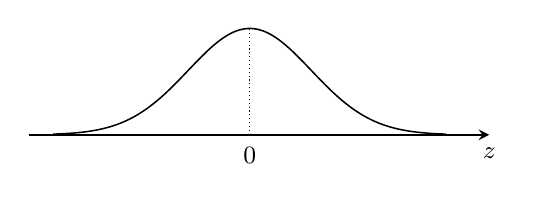
\begin{tikzpicture}[x=0.78cm, y=1.35cm, line width=0.55pt, font=\small]
  \draw[->, >=stealth, line width=0.7pt] (-3.6,0) -- (3.9,0) node[below=1pt] {$z$};
  \draw plot[domain=-3.2:3.2, samples=110, smooth] ({\x},{exp(-\x*\x/2)});
  \draw[densely dotted, line width=0.4pt] (0,0) -- (0,1);
  \node[below=1pt] at (0,0) {$0$};
\end{tikzpicture}
}\end{minipage}\par
